\subsection{Python Implementation}
	See Appendix~\ref{sec:code} for implementations of the pieces described below.
	\subsubsection{DFT}
		Our implementation of DFT doesn't use the matrix form of the equation. It uses two nested for loops, one to iterate over all $X_k$, and another to implement the summation over all $x_n$, using the standard formula. The inverse DFT is implemented in terms of the DFT, by reversing all but the first element of the input, computing the DFT and dividing all elements by the size of the input.
	\subsubsection{2D DFT}
		The 2D DFT is implemented as two separate DFTs, one over the rows, and the other over the columns. It does this by taking the DFT over the rows, transposing the matrix, doing the DFT over the rows of the result (stored in a temporary), and then returning the transpose of the result. Both the inverse and 2D discrete fourier transform implementations take a function as input. This allowed us to use one function to implement it for both the naive DFT and Cooley-Tukey.
	\subsubsection{FFT}
		Our implementation of Cooley-Tukey uses the simplest version, which only works on sets of data with a power of 2 size. It takes the input as a numpy array of complex values, uses python slicing to split into even and odd parts, recursively calling itself on each half (returning immediately when the size was 1), multiplying the odd values by the twiddle factors, and then concatenating the sum and difference of the even and odd values. The inverse and 2D discrete fourier transforms are implemented as described above.
	\subsubsection{Image Compression}
		An image consists of many thousands of pixels, so computing the transform of the entire image would be very expensive and lead to huge data loss when the high frequencies, which determine local behaviour, are removed during compression. Instead, we separate the three color channels (Red, Green, and Blue) because they are independent, and break the image into 8x8 blocks, padding as necessary. We then compute the transform of each block, dropping some fraction of the terms with the highest combined frequency (the sum of the frequencies in the vertical and horizontal directions).

\subsection{Results}
		\subsubsection{Correctness}
		\begin{figure}[h]
			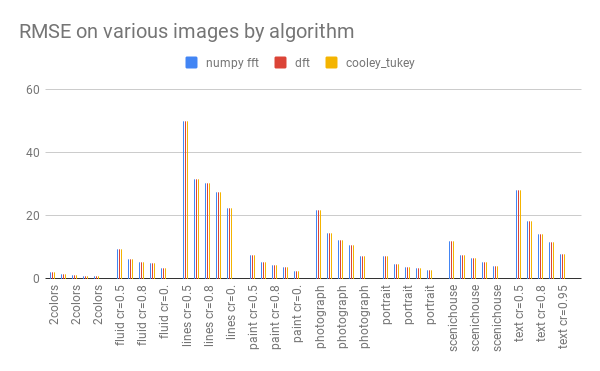
\includegraphics[width=\linewidth]{images/algorithm-accuracy.png}
			\caption{Root-mean-squared error on various images at compression rates of 0.5, 0.75, 0.8, 0.9, 0.95, and 1, where 0.5 is the most compressed (least size), and 1 is the least compressed (most size). The error at a comp. rate of 1 was effectively 0 for all images. See Appendix~\ref{sec:image-credit} for each picture.}
			\label{fig:accuracy}
		\end{figure}

		As shown in Figure~\ref{fig:accuracy}, our implementations of the discrete fourier transform, both the naive DFT and Cooley Tukey had identical accuracy to a library (numpy) FFT at various compressions. Because we used the same compression algorithm across the various implementations, this validates our code, showing that the implementations perform the same work, even if some are more optimized than others.

	\subsubsection{Performance}
		\begin{figure}[h]
			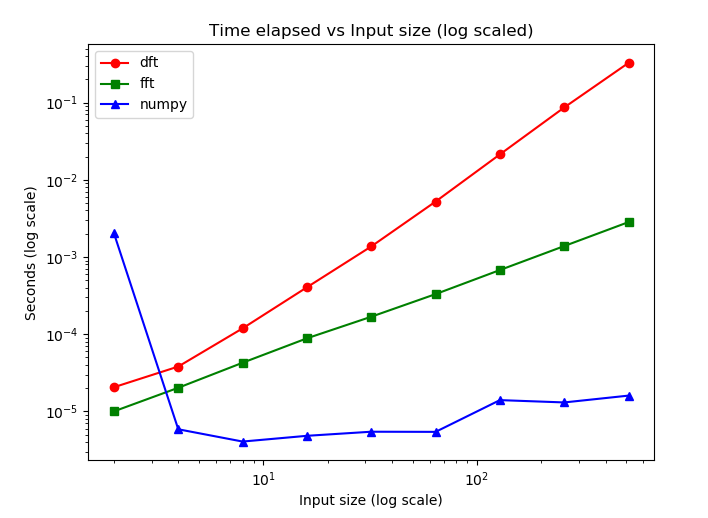
\includegraphics[width=\linewidth]{images/perfGraph.png}
			\caption{Encoding time with respect to input size for the various algorithms.}
			\label{fig:performance}
		\end{figure}
		Figure~\ref{fig:performance} shows the performance of 3 different implementations of the discrete fourier transform on several different size inputs. The red line shows the time taken by the dft algorithm, the green line shows the time taken by our implementation of Cooley-Tukey, and the blue line shows the time taken by a library implementation. Because the distance between the red and green lines grows (on a log scale), it is easy to see that the naive algorithm is asymptotically slower than Cooley-Tukey. Aside from the anomaly at the first point, the reason the blue line looks as it does is because the library implements the algorithm in C, which is far faster than Python. As a result of this, not enough data points were tested for the algorithm to display its asymptotic behavior.
	\subsubsection{Recovery Quality}
		\begin{figure}[h]
			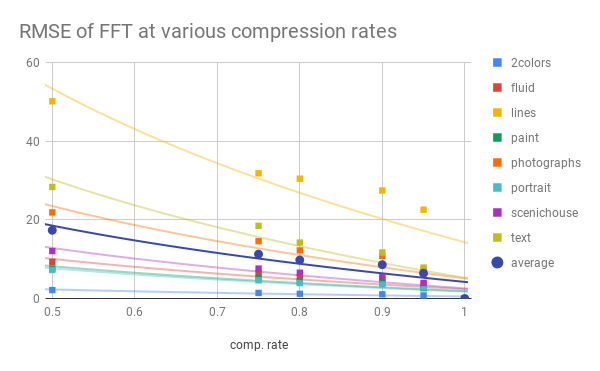
\includegraphics[width=\linewidth]{images/comprate-accuracy.png}
			\caption{Error rates of various images with respect to compression rate.}
			\label{fig:rmse-accuracy}
		\end{figure}

		\begin{figure}[h]
			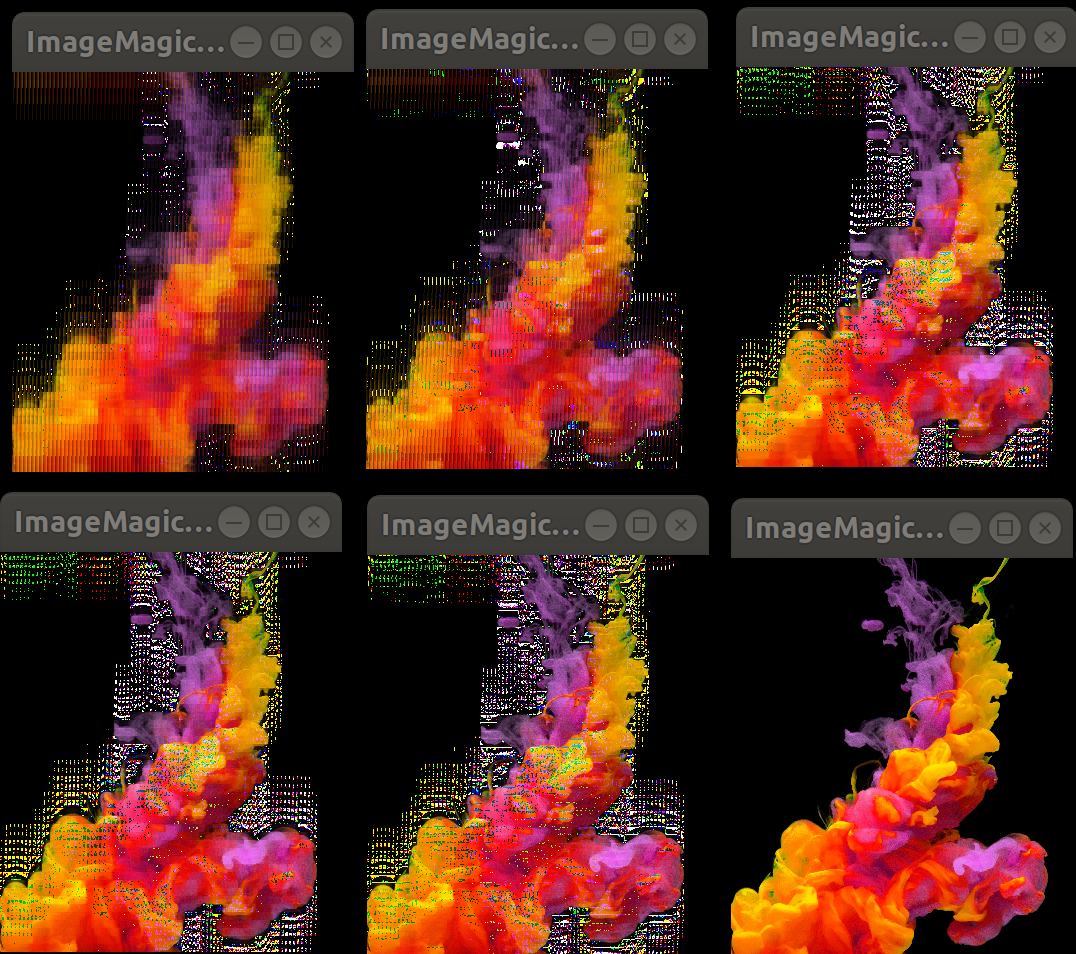
\includegraphics[width=\linewidth]{images/imgCompare1.png}
			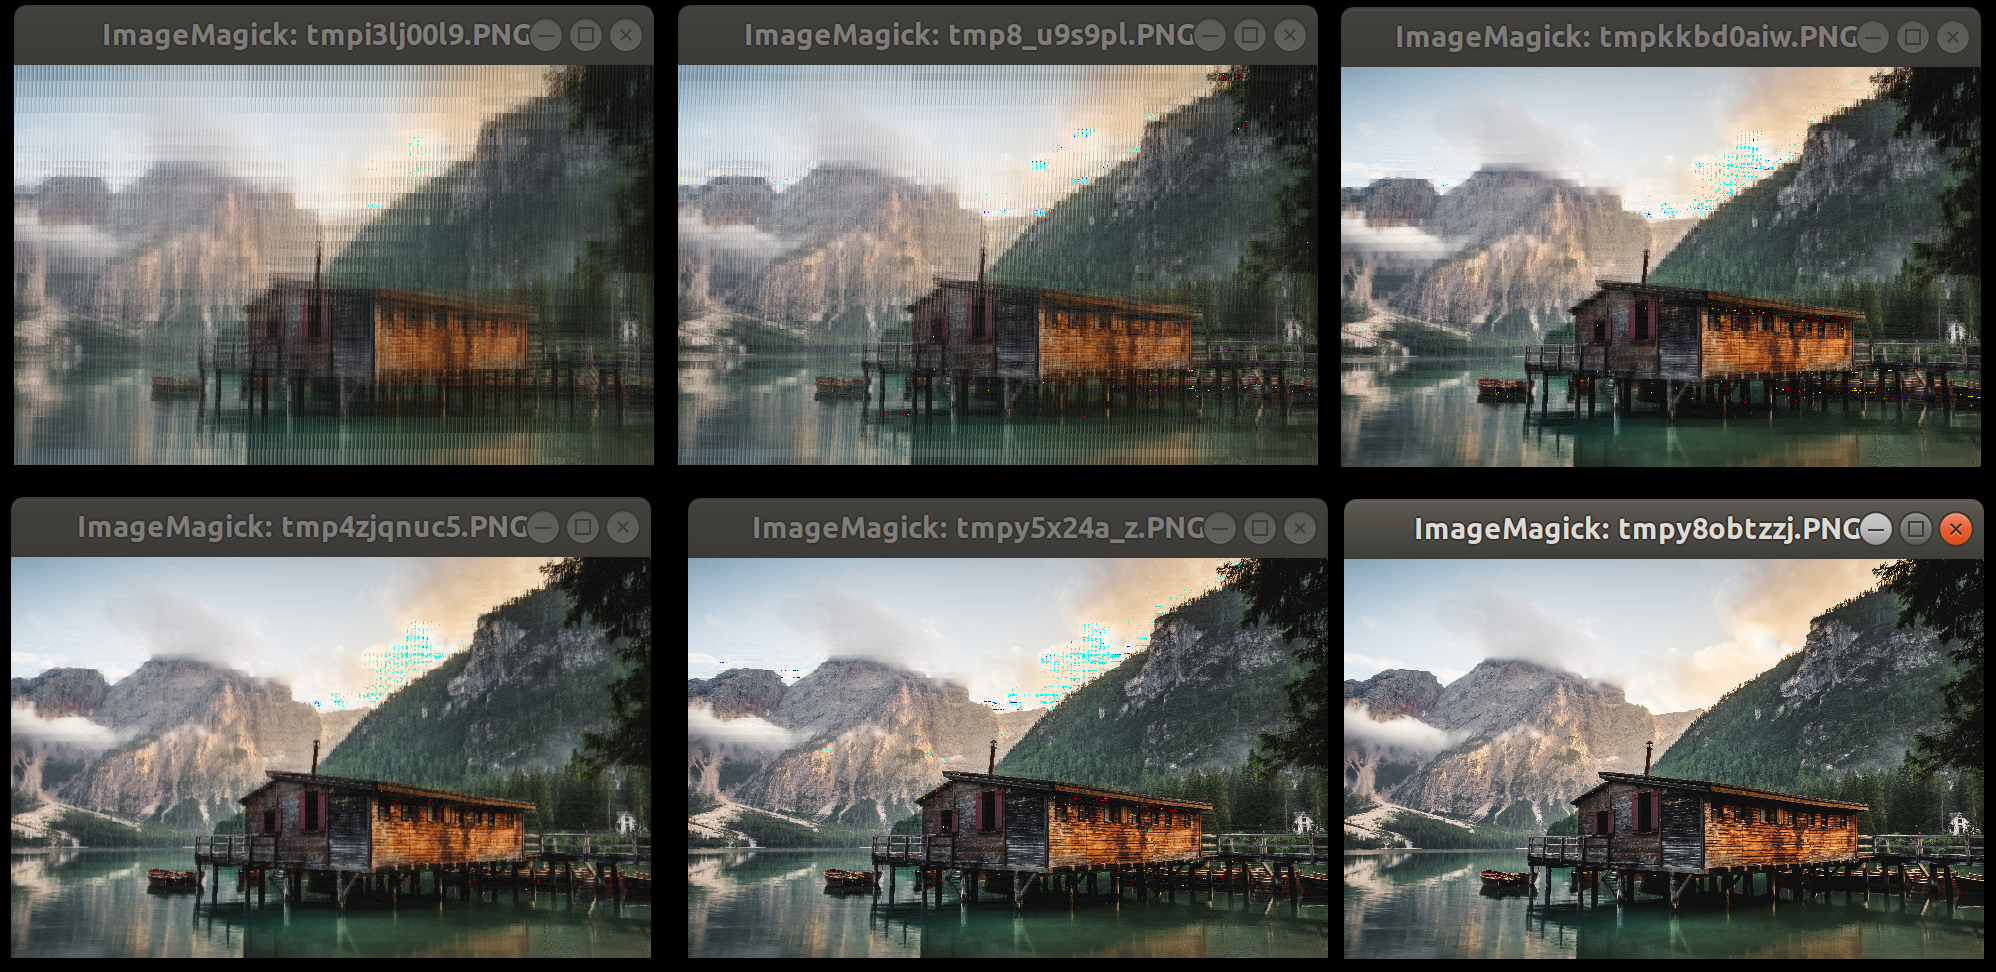
\includegraphics[width=\linewidth]{images/imgCompare2.png}
			\caption{Two images, fluid and scenichouse, compressed to 16\% (top left), 33\% (top), 50\% (top right), 66\% (bottom left), 83\% (bottom), and 100\% (bottom right) of their original size.}
			\label{fig:perceived-quality}
		\end{figure}
		Figures~\ref{fig:rmse-accuracy} and \ref{fig:perceived-quality} show the results of our compression algorithm. We compressed images to a given size, uncompressed them, and computed the root mean squared error from the original image. Even when the RMSE values aren't very large, the images can still have many artifacts, as can be easily seen on the first six images of Figure~\ref{fig:perceived-quality}. On the second six images, the compression does far better, unnoticeable at even 50\% compression. This
		difference occurs even though the original images have similar RMSE.

		Note that the metric that counts is the perceived recovery quality, not the actual accuracy. This is why JPEG uses DCT instead of DFT, and why it applies several other methods and heuristics to help maintain the appearance of accuracy. Our results do not reach industry-level perceived quality, but they do show that the FFT comes close. With additional tweaking, the human-observed error could be minimized as well.
	\subsubsection{Compression Size}
		However, even if we improve the percieved accuracy, the compression is still extremely poor, because the images actually increase in size when compressed, unless compressed to 25\% or less. This is because they are stored as floating point types instead of integers, and because a real and imaginary part must be stored, even if the highest frequencies are all ignored. To truly get JPEG-like compression, we would need to minimize our datatypes (i.e. switch to an 11-bit complex number, instead of 64), and perhaps run an additional compression step, such as a Huffman encoding or Burrows-Wheeler transform, to shrink the size further. These optimizations were omitted for time and because they do not aid in an understanding of the FFT.
